\documentclass[paper=a4,fontsize=11pt]{article}
				
\usepackage[english]{babel}
\usepackage[utf8x]{inputenc}
%% Custom colors
%%% ------------------------------------------------------------

\usepackage[svgnames]{xcolor}
\definecolor{StrongRed}{RGB}{139,0,0}
\definecolor{DarkRed}{RGB}{200,0,0}
\definecolor{awesome-red}{HTML}{DC3522}
\definecolor{header-bar}{HTML}{994C00}
\definecolor{awesome-skyblue}{HTML}{0395DE}
\definecolor{gray}{HTML}{5D5D5D}
\definecolor{lightgray}{HTML}{999999}

\usepackage[protrusion=true,expansion=true]{microtype}
\usepackage{amsmath,amsfonts,amsthm}     % Math packages
\usepackage{graphicx}                    % Enable pdflatex
\newcommand\crule[3][black]{\textcolor{#1}{\rule{#2}{#3}}}

\usepackage[margin=1in]{geometry}        % Decrease margins to 1 inch to make CV wider
%	\textheight=700px                    % Saving trees ;-)
\usepackage{url}

\usepackage[hidelinks]{hyperref}
\usepackage{geometry}
\usepackage{pdfpages}  % Permite adjuntar pdfs al final del documento
\usepackage{wrapfig}
\usepackage{lscape}
\usepackage{rotating}
\usepackage{epstopdf}
\usepackage{textcomp} % hace falta para poner apostrofe
\usepackage{array} % necesario para formatear del tiron una columna de una tabla
\usepackage{booktabs}
%\usepackage{pbox} % necesario para introducir salto de linea en celdas de una tabla
\usepackage{longtable}
\usepackage{pdflscape}
\usepackage{amsmath}
\newcommand\T{\textrm{T}}  % "true"
\newcommand\F{\textrm{F}}  % "false"
\usepackage{xspace}
\usepackage{fancyhdr}
%\setlength{\headheight}{13.6pt}

\usepackage{multicol} %lists on multicolumns side by side
\usepackage{multirow}
\usepackage{amsmath}
\usepackage{ctable}
\usepackage{adjustbox} % center images with \adjustimage
\usepackage{enumitem} % tune up itemize environment



\def\changemargin#1#2{\list{}{\rightmargin#2\leftmargin#1}\item[]}
\let\endchangemargin=\endlist  %change the margins as given by arguments



%% Font usage
%%% --------------------c----------------------------------------
\usepackage[T1]{fontenc}
\usepackage[osf]{mathpazo}


%crule\usepackage{showframe}

\frenchspacing              % Better looking spacings after periods
%\pagestyle{empty}           % No pagenumbers/headers/footers


	
%%% Macros
%%% ------------------------------------------------------------
\newlength{\spacebox}
\settowidth{\spacebox}{8888888888}			% Box to align text
\newcommand{\sepspace}{\vspace*{1em}}		% Vertical space macro

\newcommand{\MyName}[1]{ % Name
		\Huge \usefont{OT1}{phv}{b}{n} \hfill #1
		\par \normalsize \normalfont}
		
\newcommand{\MySlogan}[1]{ % Slogan (optional)
		\large \usefont{OT1}{phv}{m}{n}\hfill \textit{#1}
		\par \normalsize \normalfont}

\newcommand{\NewPart}[1]{\section*{
%\uppercase
{#1}}}


\newcommand{\Entry}[4]{
		\noindent \textbf{#1} \hfill      % Study
		\textsf{#2} \par                  % Duration
		\noindent \textit{#3} \par        % School / Institution
		  \noindent\hangindent=1em\hangafter=0 \small #4  % Description
		\normalsize \par \vspace{7.5pt}}

\newcommand{\SEntry}[3]{
		\noindent \textbf{#1} \hfill      % Study
		\textsf{#2} \par                  % Duration
		\noindent \textit{#3} \par        % School / Institution
		  \vspace{7.5pt}}
					
%Shortcuts
\newcommand{\apostrofe}{\textquotesingle\xspace}
\newcommand{\github}{\raisebox{-.25\height}{\includegraphics[width=13pt]{images/github_grey.png}}}
\newcommand{\stack}{\raisebox{-.25\height}{\includegraphics[width=13pt]{images/stack_1_grey.png}}}
\newcommand{\linkedin}{\raisebox{-.25\height}{\includegraphics[width=13pt]{images/linkedin_grey.png}}}

\newcommand{\link}{\raisebox{-.25\height}{\includegraphics[width=13pt]{images/link.png}}}

\newcommand{\mail}{\raisebox{-.25\height}{\includegraphics[width=13pt]{images/mail_grey.png}}}

\newcommand{\phone}{\raisebox{-.25\height}{\includegraphics[width=13pt]{images/phone.png}}}





%%% Custom sectioning (sectsty package)
%%% ------------------------------------------------------------
\usepackage{sectsty,regexpatch}


\makeatletter

%% Modify the look of the section rule

\newcommand{\setsectionrulecolor}[1]{\colorlet{secrulecolor}{#1}}
\setsectionrulecolor{awesome-red}% default
\xpatchcmd*{\SS@normsectionrule}% <cmd>
  {\rule}% <search>
  {\color{secrulecolor}\rule}% <replace>
  {}{}% <success><failure>
\makeatother

%% Implement the section rule
\sectionfont{%			            % Change font of \section command
	%\usefont{OT1}{phv}{b}{n}%		% bch-b-n: CharterBT-Bold font
	\sectionrule{0pt}{0pt}{-5pt}{1.7pt}} % width of section rule    
	

% Customize fancyhdr header
\fancyhf{} % sets both header and footer to nothing
\renewcommand{\headrulewidth}{0pt}
\chead{\crule[header-bar]{\textwidth}{0.5cm}}
\lfoot{}
\cfoot{}
\rfoot{}
\pagestyle{fancy}

\newcolumntype{L}[1]{>{\fontfamily{cmss}\selectfont \raggedright\let\newline\\\arraybackslash\hspace{0pt}}m{#1}}
\newcolumntype{C}[1]{>{\centering\let\newline\\\arraybackslash\hspace{0pt}}m{#1}}
\newcolumntype{R}[1]{>{\raggedleft\let\newline\\\arraybackslash\hspace{0pt}}m{#1}}


	
%%% Begin Document
%%% ------------------------------------------------------------
\begin{document}


% you can upload a photo and include it here...
%\begin{wrapfigure}{l}{0.5\textwidth}
%	\vspace*{-2em}
%		\includegraphics[width=0.15\textwidth]{photo}
%\end{wrapfigure}

%\MyName{Your Name}
%\MySlogan{Curriculum Vitae}
%
%\sepspace

\thispagestyle{fancy}



%%% Header
%%% ------------------------------------------------------------
% Set your name here
\def\name{\color{StrongRed}{\LARGE{\textsc{\textbf{Antonio Ortega Jiménez}}}}}
%\centerline{\name}
%\vspace{10pt}
%\centerline{
%Sigynsgade 79, K{\o}benhavn, Denmark
%|
%\href{mailto:ntoniogu@gmail.com}{ntoniohu@gmail.com}
%|
%\href{https://antortjim.github.io}{antortjim.github.io}
%}

\centerline{\name}

\begin{figure}[!h]
  \begin{minipage}[l]{0.15\textwidth}
  \includegraphics[width = \textwidth]{images/aoj.jpg}
 \end{minipage} %
 \begin{minipage}[l]{0.35\textwidth}
   
   \begin{itemize}[leftmargin=10pt]
     \setlength\itemsep{0.05pt}
     \large
     \item[] \mail \xspace \href{mailto:ntoniohu@gmail.com}{ntoniohu@gmail.com}
     \item[] \link \xspace \href{https://antortjim.github.io}{antortjim.github.io}
     \item[] \linkedin \xspace \href{https://www.linkedin.com/in/antortjim/en}{antortjim}
   \end{itemize}
 \end{minipage} %
 \hspace{2pt}\vrule{} \hspace{2pt}
 \begin{minipage}[r]{0.45\textwidth}
   \large
   Enthusiastic MSc. student in Bioinformatics with experience on statistical analysis and molecular biology. A passionate self-learner and hard-working person.
 \end{minipage}
\end{figure}

% Set your name here


%%% ------------------------------------------------------------
%%% End of Header

%%% Objective
%%% ------------------------------------------------------------
%\NewPart{Objective}

%Seeking the position at XXX.

%%% ------------------------------------------------------------
%%% End of Objective

%%% Skills
%%% ------------------------------------------------------------
\NewPart{Bioinformatics and Data Science skills}

\begin{itemize}
\item \textbf{Programming}: R (advanced), Python, Bash, Web development, Octave.
\item \textbf{Statistics}: Ability to develop complex models and analyse data.
\item \textbf{Data visualization}: Flair for beautiful and interactive graphics made with ggplot2 and Shiny.
\item \textbf{Biology}: Broad knowledge of biochemistry and cell biology processes.
\item \textbf{Bioinformatics}: Omics and structural data analysis experience.
\item \textbf{Computer science}: Linux and Windows OS. Git and Arduino.
\item \textbf{Reporting skills}: Strong command of Latex, Microsoft Office and Sphinx.
\end{itemize}

%%% ------------------------------------------------------------
%%% End of Skills

%%% Experience
%%% ------------------------------------------------------------
\NewPart{Experience}{}

\Entry{Bike deliverer}{Feb. 2017 - Current}{FK Distribution - Denmark}{Delivery of newspapers and commercials.}


\Entry{Volunteer assistant}{Jan. 2017 - Current}{f{\o}devareBanken - Denmark}{Assistant at both food pick up and delivery shifts around Greater Copenhagen area.}

\Entry{Assistant Research Fellow}{Nov. 2014 - Jun. 2016}{CIC Cartuja-CSIC  - Spain}{Research on cyanobacterial adaptative response to nitrogen. Work led to Bachelor Thesis.}

%%% ------------------------------------------------------------
%%% End of Experience

%%% Education
%%% ------------------------------------------------------------

\newcommand{\kulogo}{ \hspace{5pt} \includegraphics[width=30pt]{images/ku_logo.png}}
\newcommand{\uslogo}{ \hspace{5pt} \includegraphics[width=30pt]{images/us_logo.png}}
\newcommand{\msctitle}{%\begin{tabular}[c]{@{}c@{}}
                       \textbf{MSc.} %\\
                       \textbf{Bioinformatics}
                       %\end{tabular}
                       }


\newcommand{\bsctitle}{\textbf{BSc. Biochemistry}}
\newcommand{\bscyears}{\begin{math}\boldsymbol{2012-2016}\end{math}}
\newcommand{\mscyears}{\begin{math}\boldsymbol{2016-2018}\end{math}}		


\NewPart{Education}{}



\begin{table}[!h]
\begin{tabular}{C{50pt} R{100pt} l}
\multirow{3}{*}{\kulogo}      & \msctitle                           & \mscyears     \\
                              & \textit{K{\o}benhavns Universitet}  & \small{Honors on Biological Sequence Analysis.}              \\ 
                              & Denmark                             &     \\  % Insertar entre & y // la GPA del master
                              &                                     &               \\ 
\multirow{4}{*}{\uslogo}      & \bsctitle                           &  \bscyears    \\
                              & \textit{Universidad de Sevilla}     &  \small{4 Honors including Bioinformatics, Genetics and Statistics.}    \\
                              & Spain                               &  \small{\textbf{GPA}: \begin{math}3.38/4.0\end{math}.} \\

\end{tabular}
\end{table}

%%% ------------------------------------------------------------
%%% End of Education


%%% Portfolio
%%% ------------------------------------------------------------
\NewPart{Portfolio}

A listing of relevant projects may be found at \href{https://antortjim.github.io/portfolio/}{https://antortjim.github.io/portfolio/}.

%%% ------------------------------------------------------------
%%% End of Portfolio

%%% Awards
%%% ------------------------------------------------------------

\NewPart{Awards}{}

\Entry{Best Huelva province high-school record}{Jun. 2012}{Government of Andalusia}{
The two best high school students from the province of Huelva were awarded this prize.}
\sepspace

\Entry{Winner at the high school mathematics olympics}{Apr. 2008}{Andalusian Association for Mathematical Education THALES}{Students were asked to solve non trivial mathematical problems using logic and imagination.}

%%% ------------------------------------------------------------
%%% End of Awards

%%% Languages
%%% ------------------------------------------------------------
\NewPart{Languages}

\begin{multicols}{2}

\begin{itemize}
\item \textbf{Spanish}: Native
\item \textbf{English}: Proficient (C1 level)
\end{itemize}

\columnbreak

\begin{itemize}
\item \textbf{French}: Elementary (B1)
\item \textbf{Danish}: Beginner (Currently learning)
\end{itemize}

\end{multicols}
%%% ------------------------------------------------------------
%%% End of Languages

\thispagestyle{empty}
	

%%% Independent learning
%%% ------------------------------------------------------------
\NewPart{Complementary education}{}


\SEntry{Summer School on Bioinformatics}{July 2015}{Universidad Complutense de Madrid} 
  
\SEntry{Machine Learning by Andrew Ng}{July 2016}{University of Stanford at Coursera}

%%% ------------------------------------------------------------
%%% End of Independent learning

%%% Hobbies
%%% ------------------------------------------------------------
\NewPart{Hobbies}
I attend weekly sessions of strength training at USG, the University's sports center, because I think keeping active is really important. I love cykling around Copenhagen. In my free time I enjoy learning languages and exchanging culture with people around me. For this reason, I signed up for Danish lessons at KU. This way I am slowly getting in touch with the Danish lifestyle.

%%% ------------------------------------------------------------
%%% End of Hobbies


\vfill
\textcolor{lightgray}{Transcript of results from K{\o}benhavns Universitet}


% Motivation letter
%\hypertarget{motivation}{}
%\includepdf[pages={1,2}]{carta/Antonio_Ortega_Motivation_Letter.pdf}
%\clearpage


% KU transcript

%\thispagestyle{empty}
\newgeometry{margin=20pt, bottom=5pt}
\hypertarget{KU_transcript}{}
\centering
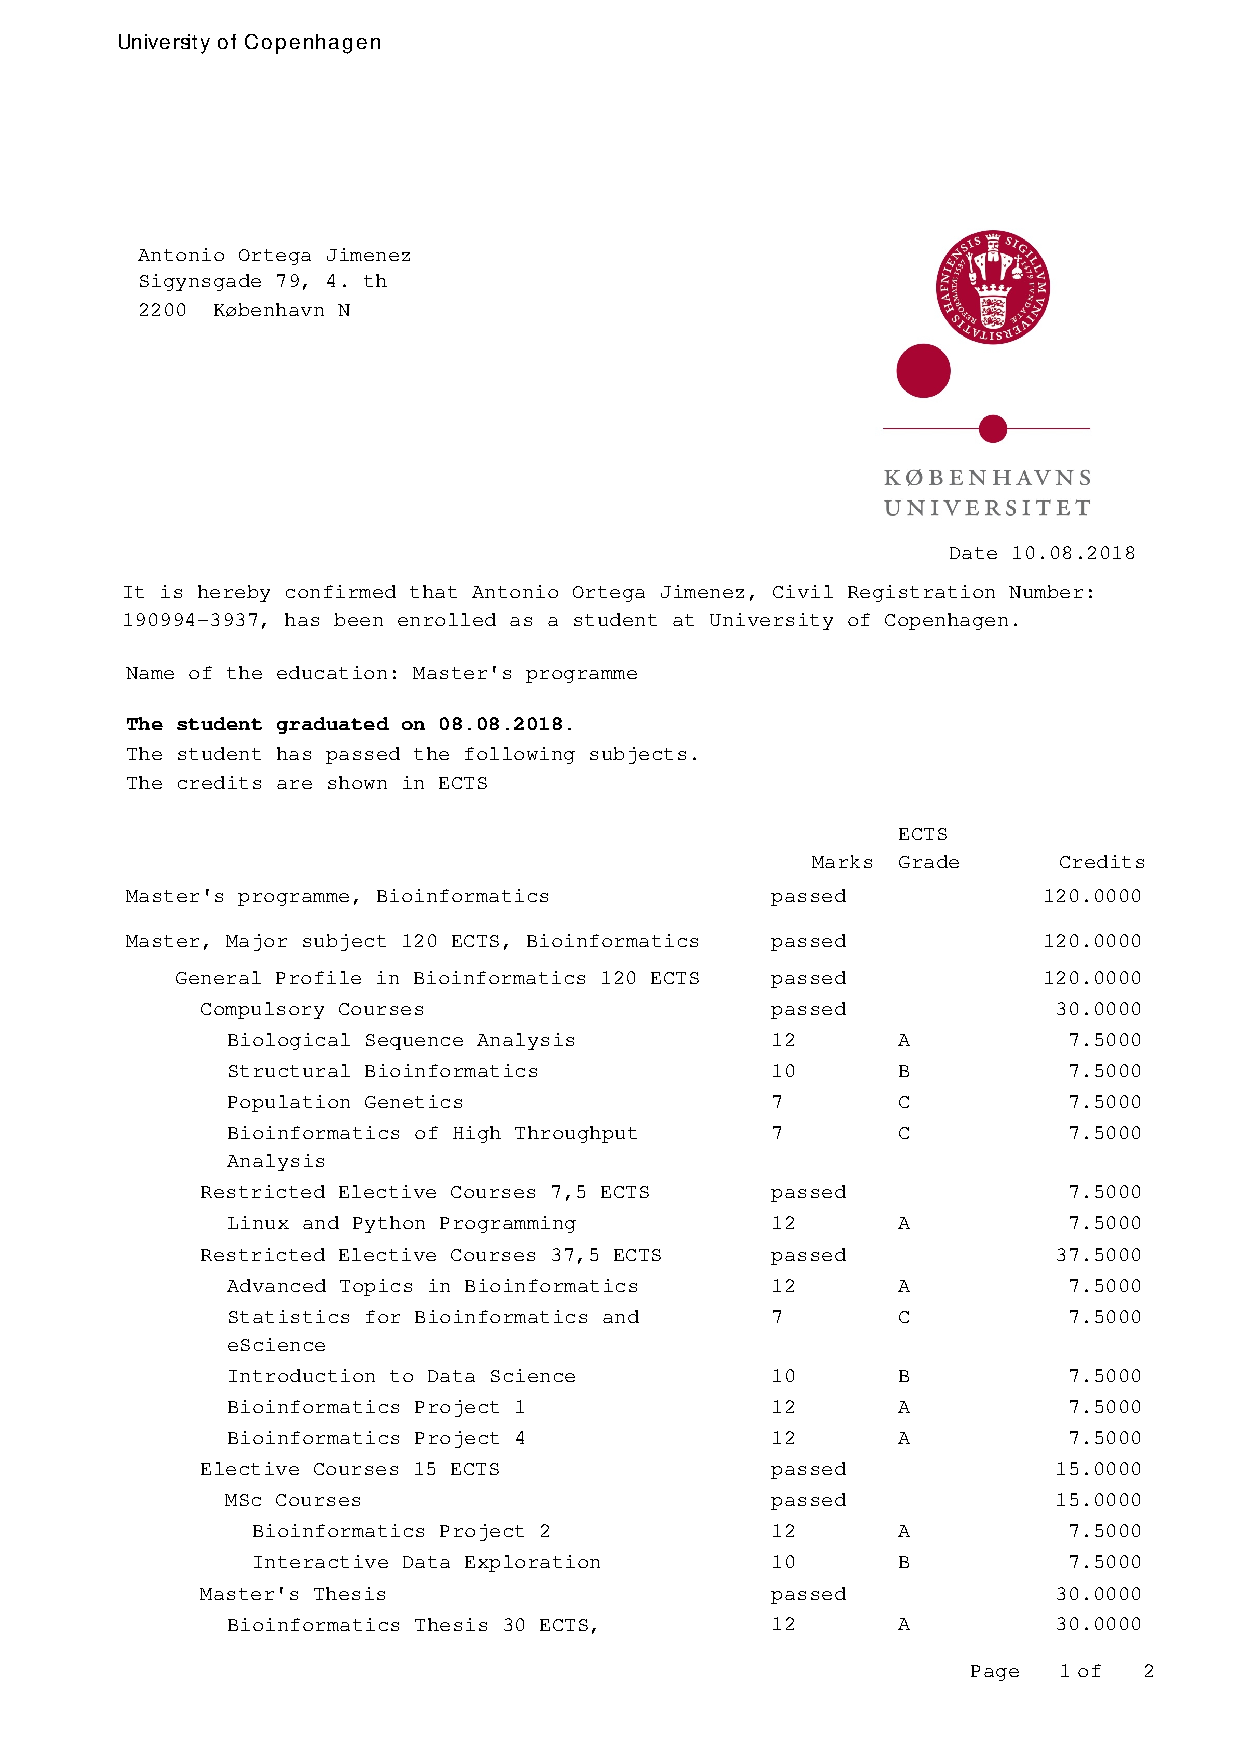
\includegraphics[scale=0.9]{append/transcript.pdf}
\clearpage


%% Diploma del premio extraordinario
%
%%\thispagestyle{empty}
%\newgeometry{margin=20pt, bottom=5pt}
%\hypertarget{premio_extraordinario}{}
%\begin{landscape}
%\centering
%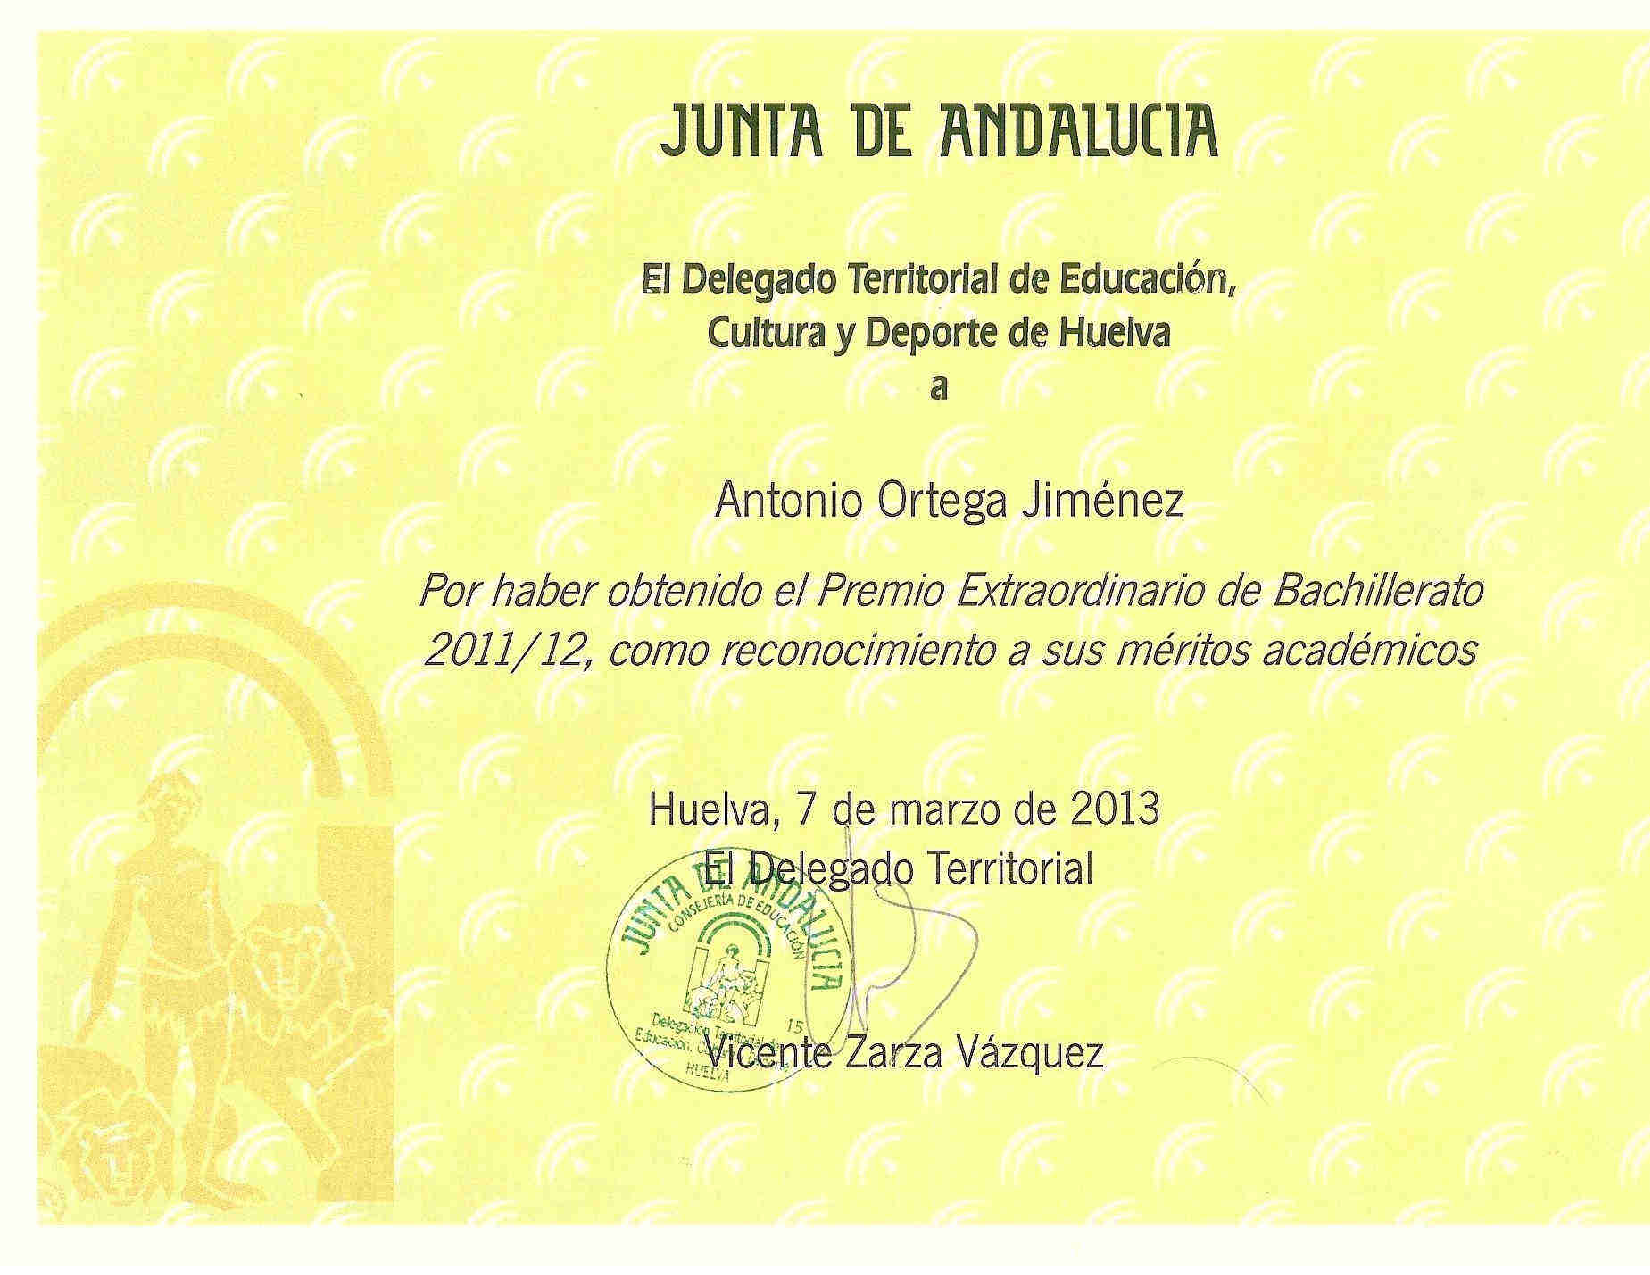
\includegraphics[scale=0.9]{append/premio_extraordinario.pdf}
%\end{landscape}
%\restoregeometry
%\clearpage
%
%
%% Diploma del curso de bioinformatica en la complu
%\thispagestyle{empty}
%
%\newgeometry{margin=20pt, bottom=5pt}
%\hypertarget{complu}{}
%\begin{landscape}
%\centering
%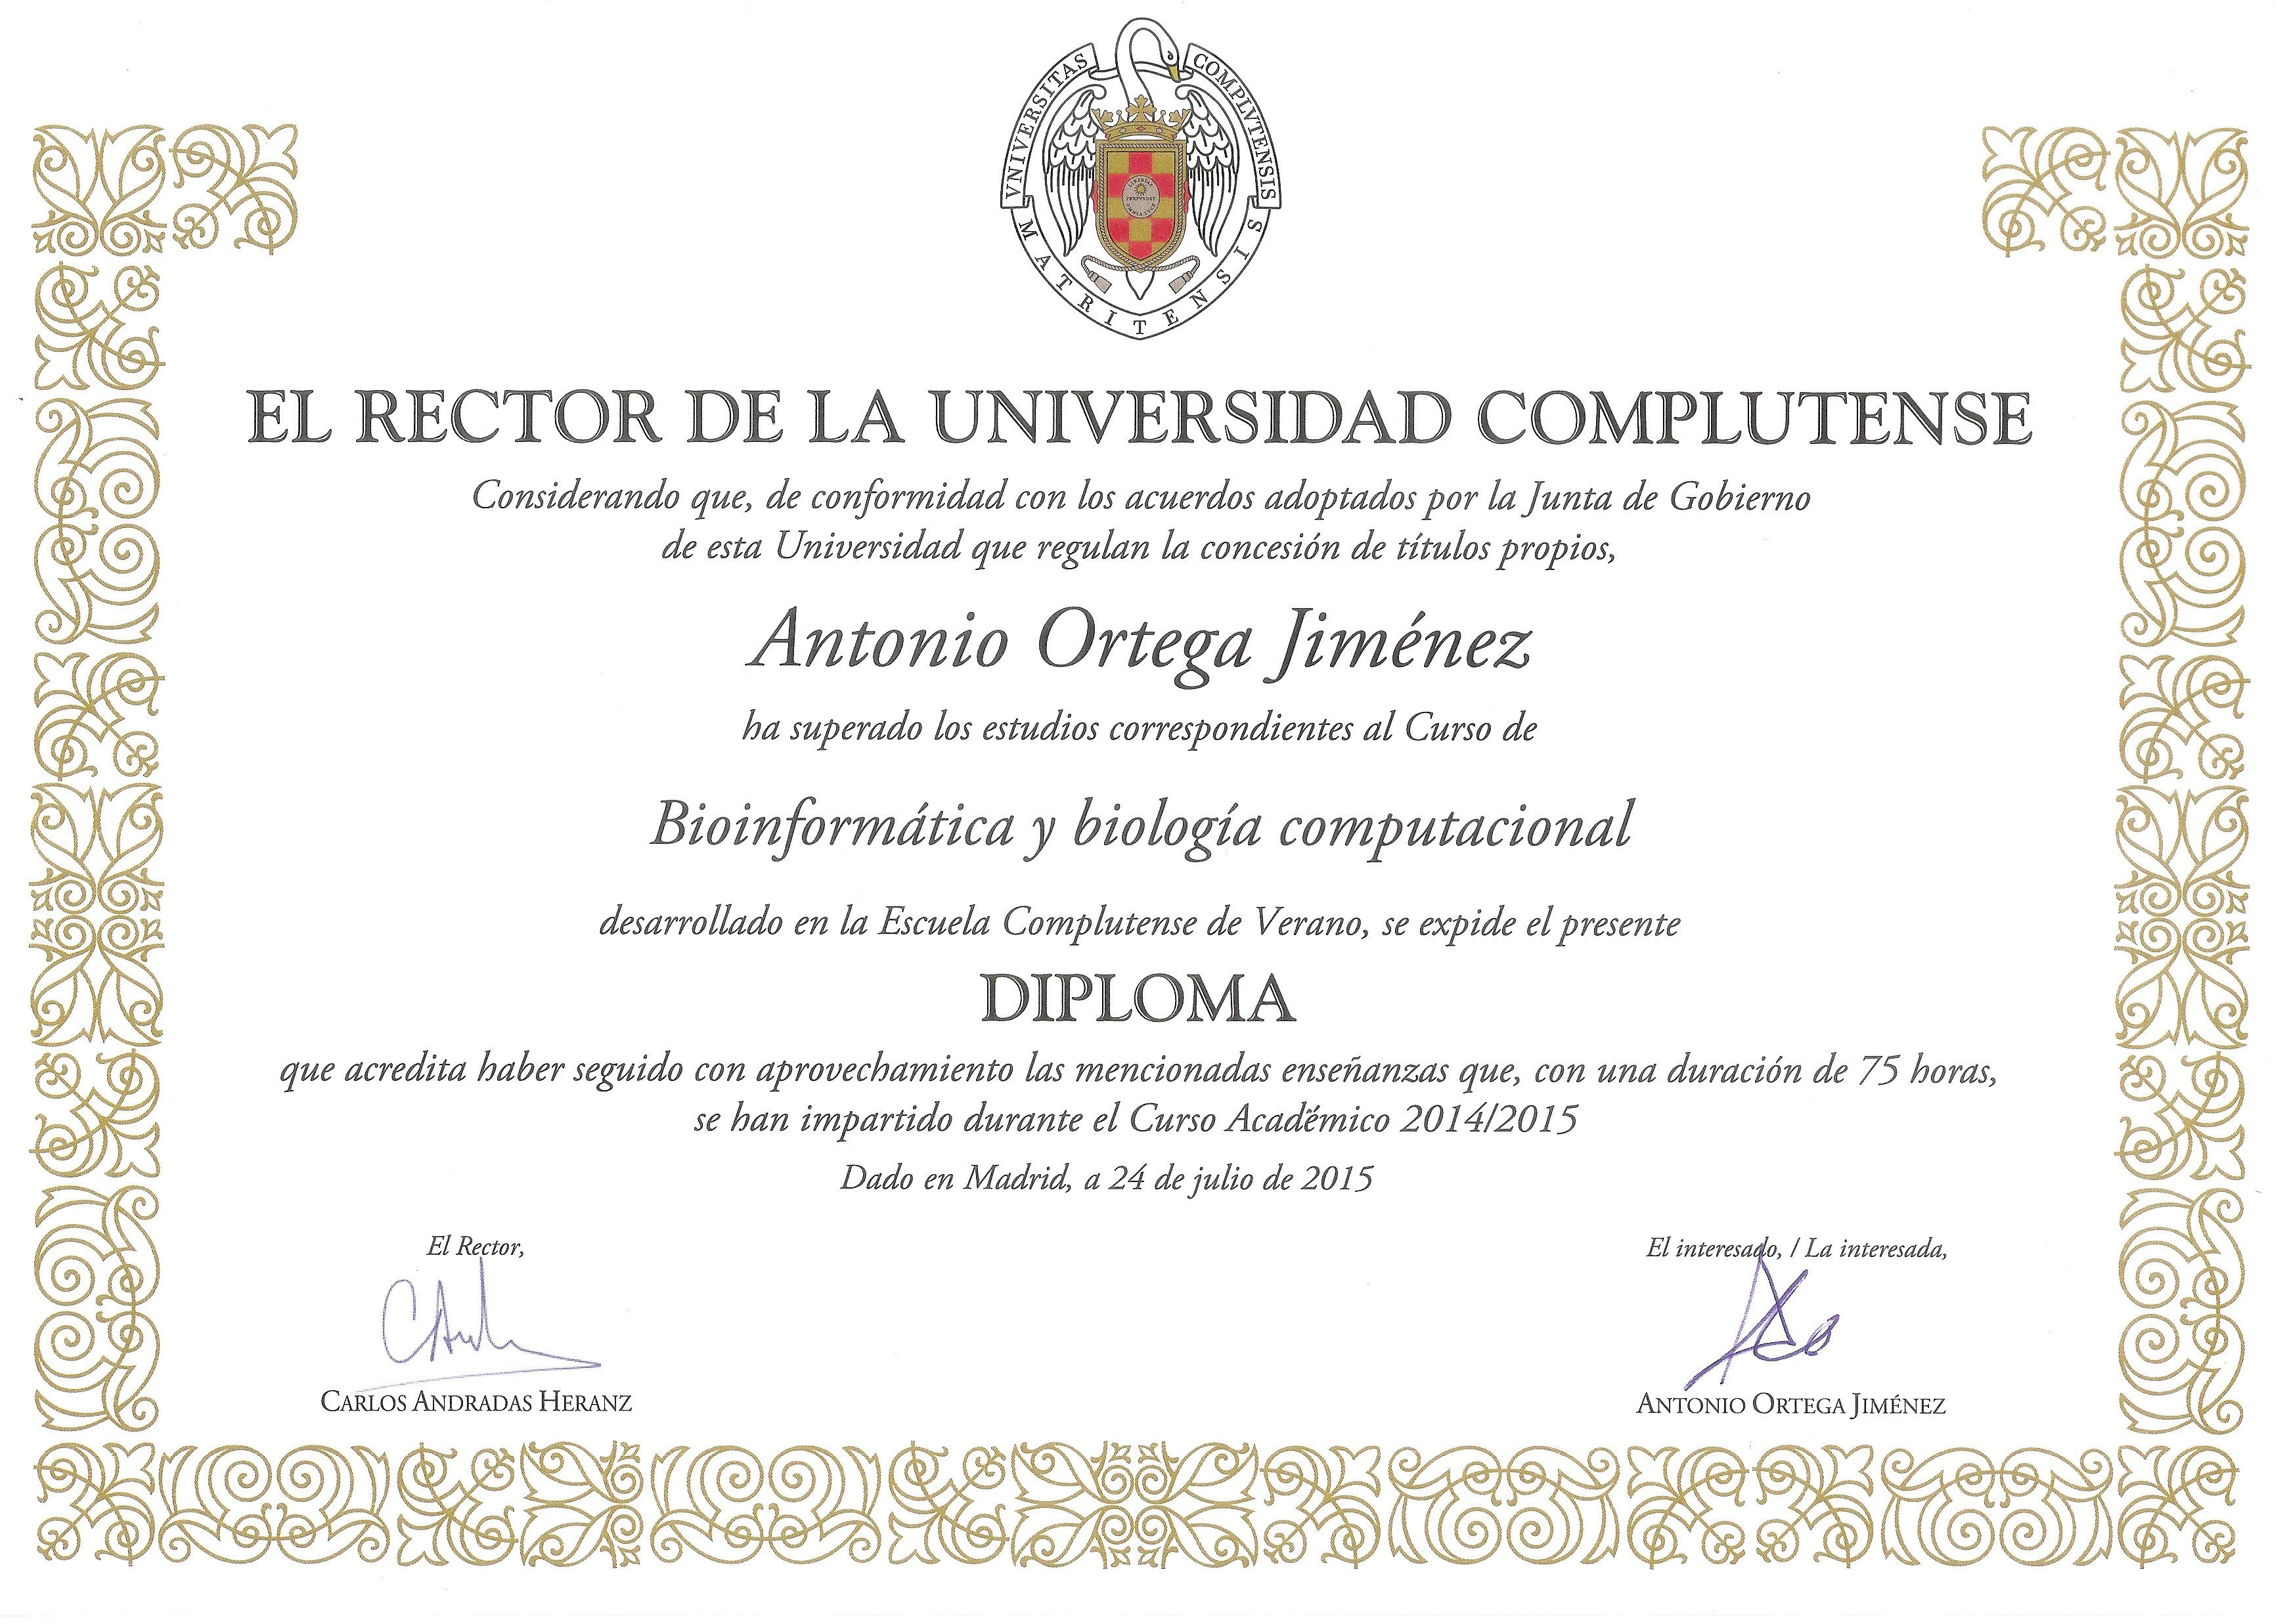
\includegraphics[scale=0.2]{append/bioinformatica2.jpg}
%\end{landscape}
%\restoregeometry
%\clearpage
%
%
%\newgeometry{margin=20pt, bottom=5pt}
%\hypertarget{ML-Coursera}{}
%\begin{landscape}
%\centering
%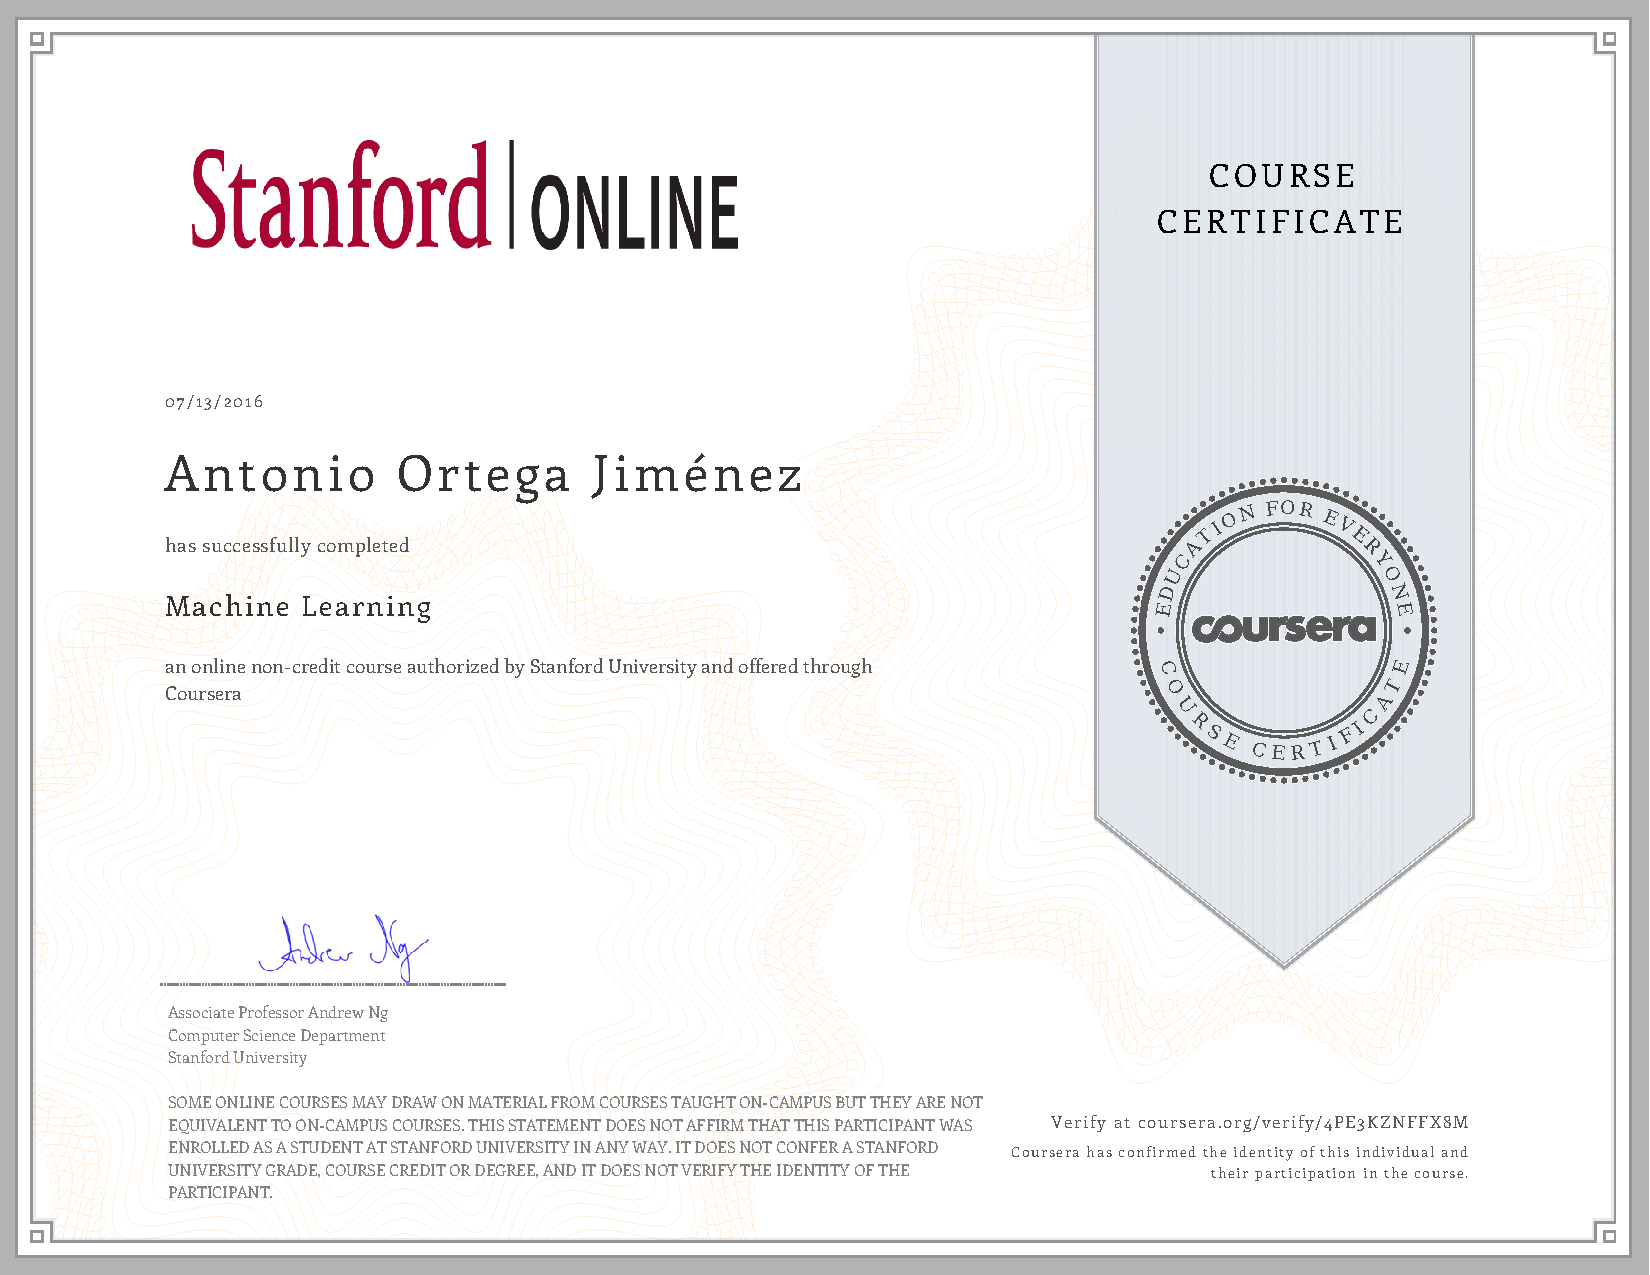
\includegraphics[width=\textwidth]{ML-Coursera.pdf}
%\end{landscape}
%\restoregeometry
%\clearpage
%
%
%%Expediente oficial en inglés
%\hypertarget{exp-en}{}
%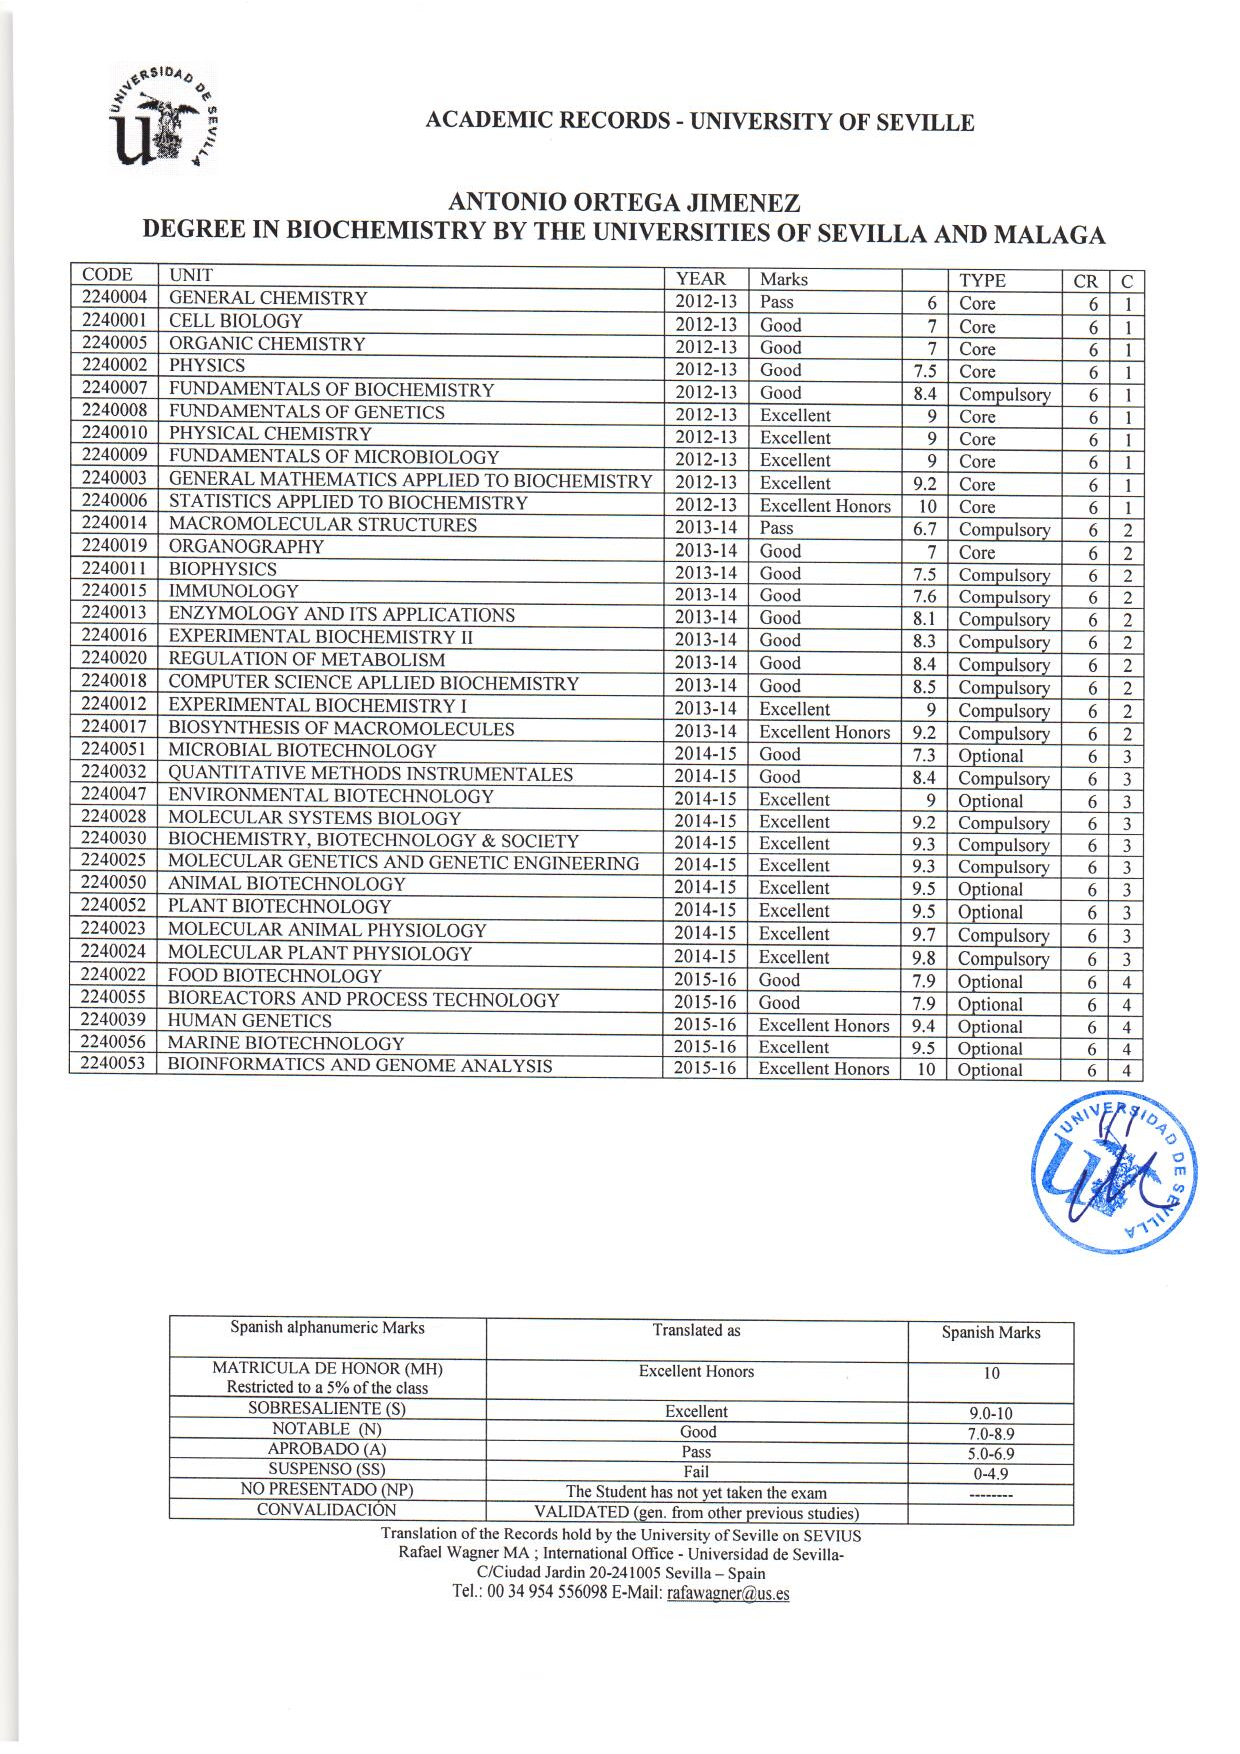
\includepdf[pages={1}]{Transcript-English.pdf}
%\clearpage
%
%
%\hypertarget{cae}{}
%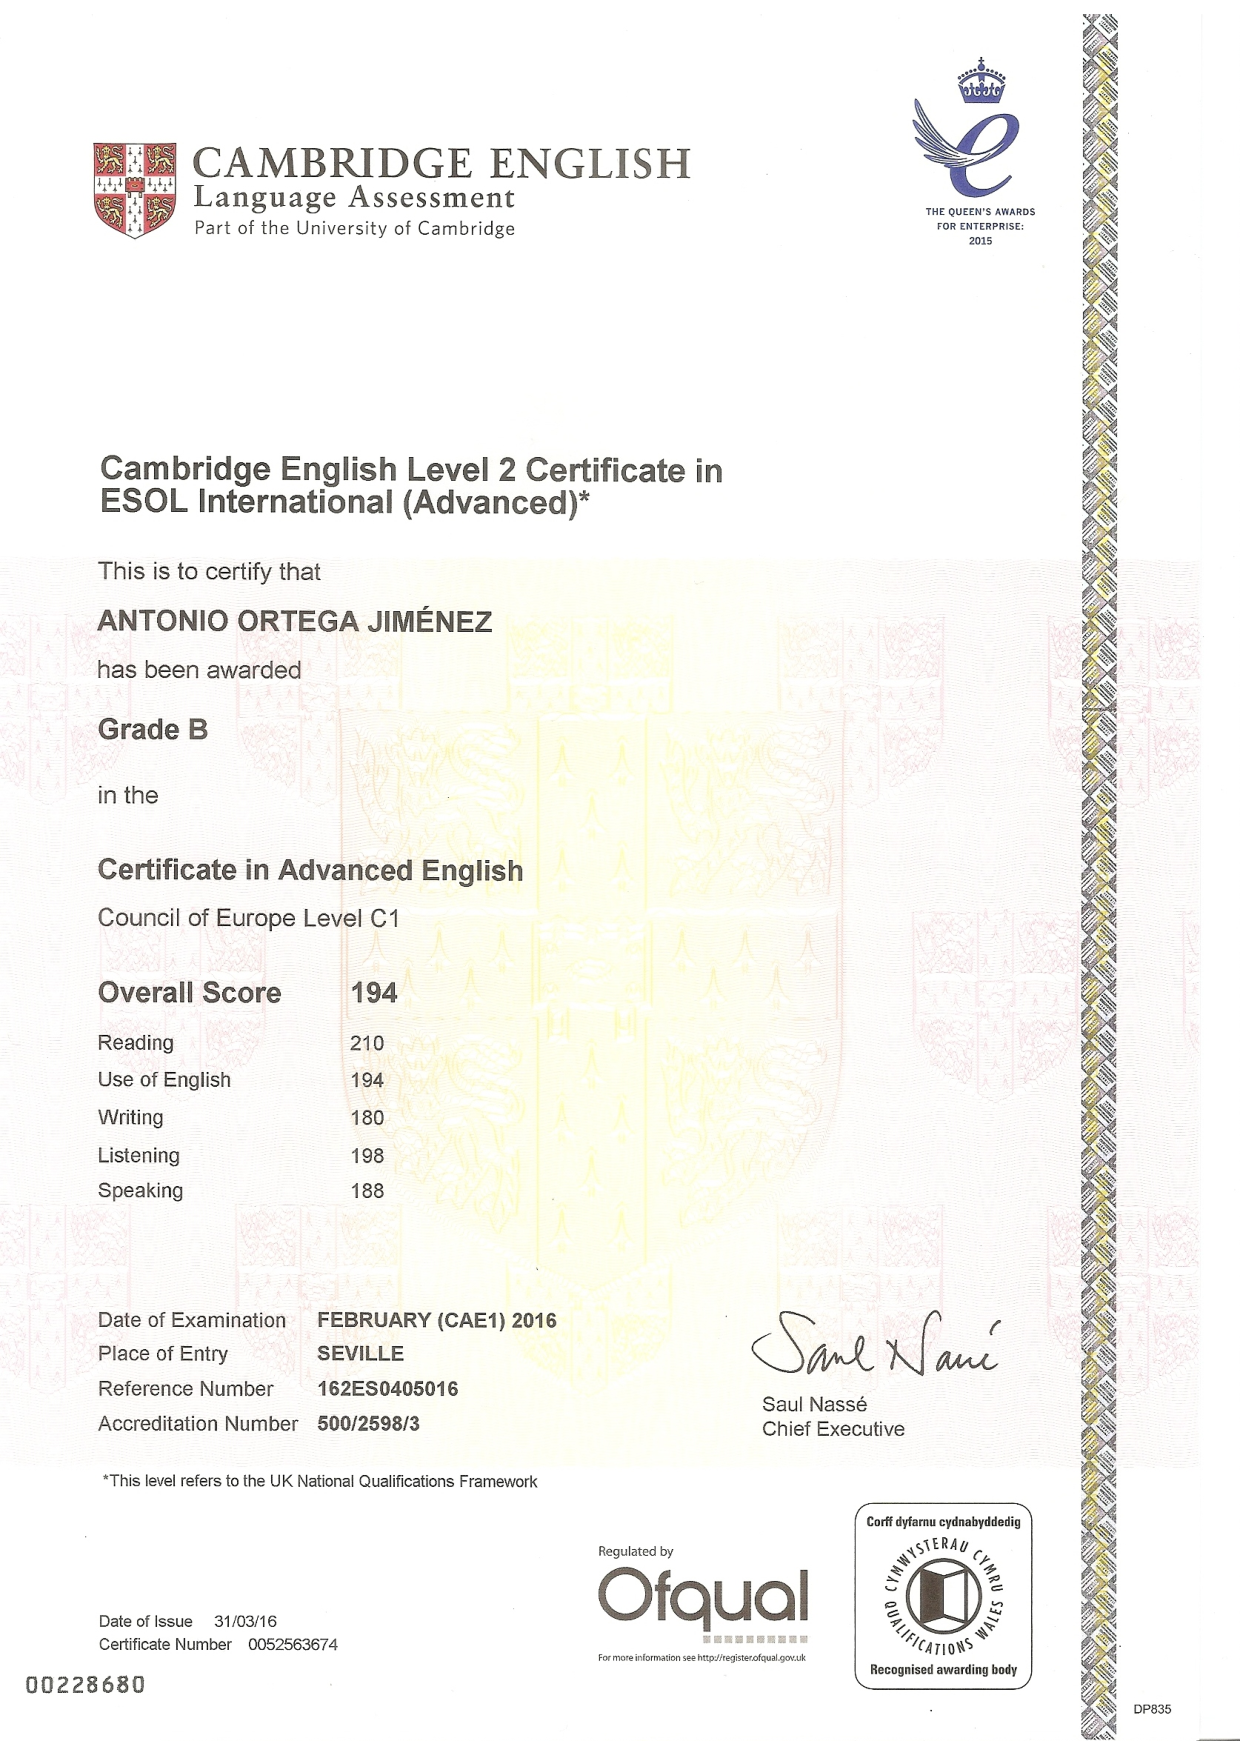
\includepdf{cae.pdf}
%\clearpage



%Certificado DELF
%\thispagestyle{empty}
%\begin{landscape}
%\begin{figure}
%\hspace{-2.5 cm}
%\includegraphics[scale=0.3]{append/delf.jpg}
%\end{figure}
%\end{landscape}
%\clearpage
\end{document}
